\chapter{高等数学：凹凸性}

\section{凹凸性}

\begin{problemblock}
\textbf{例1.} 设任意阶可导函数 \(f(x)\) 的图形如图所示，则下列 Taylor 展开式
\[
\text{① }x+\frac12x^2+\frac16x^3+R_1;
\]
\[
\text{② }1-\frac1{2!}(x-x_1)-\frac1{4!}(x-x_1)^2+R_2;
\]
\[
\text{③ }1+\frac12(x-x_2)+\frac13(x-x_2)^2+R_3.
\]
其中 \(R_1,R_2,R_3\) 均为 Taylor 展开式的余项，可能是 \(f(x)\) 的 Taylor 展开式的个数为（\quad）

A. \(0\)\qquad B. \(1\)\qquad C. \(2\)\qquad D. \(3\)

\begin{center}
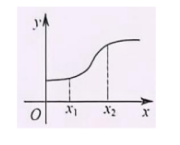
\includegraphics[width=.32\textwidth]{figures/gaoshu/page_050_graph.png}
\end{center}
\end{problemblock}
\begin{solutionblock}
\analysis{Taylor 多项式的常数项、一次项、二次项分别反映该点的函数值、切线斜率与凹凸性。逐项和图形对照即可。}
① 若是 \(x=0\) 处展开，则常数项为 \(0\)，即应有 \(f(0)=0\)。但图像在 \(x=0\) 附近函数值为正，不经过原点，因此①不可能。

② 若是在 \(x=x_1\) 处展开，则一次项系数为 \(-\frac1{2!}<0\)，表示
\[
f'(x_1)<0.
\]
但图像在 \(x_1\) 附近单调增加，切线斜率非负，故②不可能。

③ 若是在 \(x=x_2\) 处展开，则二次项系数为 \(\frac13>0\)，表示
\[
\frac{f''(x_2)}2=\frac13,\qquad f''(x_2)>0.
\]
但图像在 \(x_2\) 附近已向下弯，呈凹向下形态，故 \(f''(x_2)<0\)，③也不可能。

所以三个式子都不可能。
\answer{A}
\examnote{图像与 Taylor 系数对应：常数项看函数值，一次项看斜率，二次项看凹凸。}
\end{solutionblock}

\begin{problemblock}
\textbf{例2.} 设 \(f(x)\) 在 \([0,1]\) 上二阶可导，
\[
\int_0^1 f(x)\,dx=0,
\]
则下列说法中正确的是（\quad）
\begin{enumerate}[label=\Alph*., leftmargin=2.2em]
\item 若 \(f''(x)>0\)，则 \(f\left(\frac12\right)>0\)；
\item 若 \(f''(x)\ge0\)，则 \(f(x)\ge f(1)x+f(0)(1-x)\)；
\item 若 \(f''(x)<0\)，则 \(\dfrac{f(0)+f(1)}2<0\)；
\item 若 \(f''(x)<0\)，则对任意 \(x_1<x_2<x_3\)，有
\[
\frac{f(x_1)-f(x_2)}{x_1-x_2}
<
\frac{f(x_2)-f(x_3)}{x_2-x_3}.
\]
\end{enumerate}
\end{problemblock}
\begin{solutionblock}
\analysis{本题考查 Hermite-Hadamard 不等式与割线斜率。\(f''>0\) 是凸，\(f''<0\) 是凹。}
若 \(f''>0\)，则 \(f\) 为严格凸函数。Hermite-Hadamard 不等式给出
\[
f\left(\frac12\right)<\int_0^1 f(x)\,dx=0,
\]
故 A 错。

若 \(f''\ge0\)，凸函数图像在端点弦下方，即
\[
f(x)\le f(1)x+f(0)(1-x),
\]
故 B 的不等号方向反了。

若 \(f''<0\)，则 \(f\) 为严格凹函数，图像在端点弦上方，于是
\[
\int_0^1 f(x)\,dx>\frac{f(0)+f(1)}2.
\]
由题设积分为 \(0\)，得
\[
0>\frac{f(0)+f(1)}2,
\]
故 C 正确。

若 \(f''<0\)，导函数单调减少，割线斜率也随区间右移而减少，因此应有左侧割线斜率大于右侧割线斜率，D 的方向错误。
\answer{C}
\examnote{凹凸函数的积分平均、端点平均、中点值之间有固定大小关系。}
\end{solutionblock}

\begin{problemblock}
\textbf{例3.} 已知 \(f(x)\) 为二阶可导的正值函数，
\[
f(0)=f'(0)=1,\qquad f(x)f''(x)\ge [f'(x)]^2,
\]
则（\quad）
\begin{enumerate}[label=\Alph*., leftmargin=2.2em]
\item \(f(2)\le e^2\le\sqrt{f(1)f(3)}\)；
\item \(e^2\le f(2)\le\sqrt{f(1)f(3)}\)；
\item \(\sqrt{f(1)f(3)}\le e^2\le f(2)\)；
\item \(\sqrt{f(1)f(3)}\le f(2)\le e^2\)。
\end{enumerate}
\end{problemblock}
\begin{solutionblock}
\analysis{条件 \(ff''\ge(f')^2\) 正好说明 \((\ln f)''\ge0\)，即 \(\ln f\) 为凸函数。}
令
\[
u(x)=\ln f(x).
\]
因为 \(f(x)>0\)，有
\[
u''(x)=\frac{f(x)f''(x)-[f'(x)]^2}{f^2(x)}\ge0.
\]
所以 \(u\) 是凸函数。又
\[
u(0)=\ln f(0)=0,\qquad
u'(0)=\frac{f'(0)}{f(0)}=1.
\]
凸函数在切线上方，故
\[
u(2)\ge u(0)+u'(0)\cdot2=2,
\]
即
\[
f(2)\ge e^2.
\]
另一方面，\(2\) 是 \(1\) 与 \(3\) 的中点，由凸性
\[
u(2)\le\frac{u(1)+u(3)}2.
\]
两边取指数得
\[
f(2)\le\sqrt{f(1)f(3)}.
\]
因此
\[
e^2\le f(2)\le\sqrt{f(1)f(3)}.
\]
\answer{B}
\examnote{遇到 \(ff''\ge(f')^2\)，优先令 \(u=\ln f\)。}
\end{solutionblock}

\begin{problemblock}
\textbf{例4.} 设 \(f(x)\) 在 \([-1,1]\) 上二阶可导，且
\[
f''(x)>0,\qquad
\lim_{x\to0}\frac{x}{f(x)+1}=e^a.
\]
记
\[
I=\int_{-1}^1 f(x)\,dx,
\]
则（\quad）

A. \(I>a\)\qquad B. \(I>-2\)\qquad C. \(I=0\)\qquad D. \(I=a\)
\end{problemblock}
\begin{solutionblock}
\analysis{先由极限推出 \(f(0)=-1\) 与 \(f'(0)=e^{-a}\)，再用凸函数在切线上方。}
因为
\[
\lim_{x\to0}\frac{x}{f(x)+1}=e^a
\]
为有限非零数，必须有
\[
f(0)+1=0,\qquad f(0)=-1.
\]
又
\[
f(x)+1=f(x)-f(0)\sim f'(0)x,
\]
所以
\[
\frac{x}{f(x)+1}\to\frac1{f'(0)}=e^a,
\qquad f'(0)=e^{-a}.
\]
由 \(f''(x)>0\)，\(f\) 严格凸，因此对 \(x\ne0\)，
\[
f(x)>f(0)+f'(0)x=-1+e^{-a}x.
\]
积分得
\[
I=\int_{-1}^{1}f(x)\,dx
>
\int_{-1}^{1}(-1+e^{-a}x)\,dx
=-2.
\]
\answer{B}
\examnote{凸函数大于其切线；凹函数小于其切线。}
\end{solutionblock}

\begin{problemblock}
\textbf{例5.} 设
\[
f'(x)>0,\qquad f''(x)<0,\qquad x>0.
\]
对任意正整数 \(n\)，记
\[
I_1=\frac12[f(n+1)-f(n)],
\]
\[
I_2=f(n)-f\left(\frac{2n-1}{2}\right),\qquad
I_3=f\left(\frac{2n+1}{2}\right)-f(n).
\]
则（\quad）

A. \(I_1>I_2>I_3\)\quad
B. \(I_1>I_3>I_2\)\quad
C. \(I_2>I_1>I_3\)\quad
D. \(I_2>I_3>I_1\)
\end{problemblock}
\begin{solutionblock}
\analysis{\(f'>0\) 表示增函数，\(f''<0\) 表示导数递减，所以等长区间上的增量随区间右移而减小。}
三个量都与长度为 \(\frac12\) 的增量有关：
\[
I_2=f(n)-f\left(n-\frac12\right),
\]
\[
I_3=f\left(n+\frac12\right)-f(n),
\]
并令
\[
J=f(n+1)-f\left(n+\frac12\right).
\]
由于 \(f''<0\)，\(f'\) 递减，所以等长区间上的函数增量随区间右移而递减：
\[
I_2>I_3>J.
\]
又
\[
I_1=\frac12[f(n+1)-f(n)]
=\frac12(I_3+J).
\]
因为 \(I_3>J\)，故
\[
I_3>I_1>J.
\]
综上
\[
I_2>I_3>I_1.
\]
\answer{D}
\examnote{凹函数的“边际增量”递减；等长小区间越靠右，增量越小。}
\end{solutionblock}

\begin{problemblock}
\textbf{例6.} 若 \(f(x)\) 为区间 \(I\) 上的连续函数，且 \(f(x)\) 的值域包含于 \(I\)，\(x_1,x_2\) 为 \(I\) 中任意两个不同点，则下列说法正确的是（\quad）
\begin{enumerate}[label=\Alph*., leftmargin=2.2em]
\item 若在区间 \(I\) 上 \(f(x)<0,f''(x)>0\)，则
\[
f^2\left(\frac{x_1+x_2}{2}\right)
<\frac{f^2(x_1)+f^2(x_2)}2;
\]
\item 若在区间 \(I\) 上 \(f'(x)<0,f''(x)>0\)，则
\[
f^2\left(\frac{x_1+x_2}{2}\right)
<\frac{f^2(x_1)+f^2(x_2)}2;
\]
\item 若在区间 \(I\) 上 \(f(x)>0,f''(x)>0\)，则
\[
f\left[f\left(\frac{x_1+x_2}{2}\right)\right]
<\frac{f[f(x_1)]+f[f(x_2)]}{2};
\]
\item 若在区间 \(I\) 上 \(f'(x)>0,f''(x)>0\)，则
\[
f\left[f\left(\frac{x_1+x_2}{2}\right)\right]
<\frac{f[f(x_1)]+f[f(x_2)]}{2}.
\]
\end{enumerate}
\end{problemblock}
\begin{solutionblock}
\analysis{本题考查复合函数的凸性。若 \(f'>0,f''>0\)，则 \(f\) 增且凸，复合函数 \(f\circ f\) 仍凸。}
在 D 的条件下，
\[
(f\circ f)'(x)=f'(f(x))f'(x),
\]
\[
(f\circ f)''(x)
=f''(f(x))[f'(x)]^2+f'(f(x))f''(x).
\]
由于 \(f(x)\in I\)，且 \(f'(x)>0,f''(x)>0\) 在 \(I\) 上成立，所以
\[
(f\circ f)''(x)>0.
\]
因此 \(f\circ f\) 为严格凸函数，由凸函数中点不等式，
\[
f\left[f\left(\frac{x_1+x_2}{2}\right)\right]
<
\frac{f[f(x_1)]+f[f(x_2)]}{2}.
\]
D 正确。

A、B 中讨论 \(f^2\) 的凸性，但
\[
(f^2)''=2(f')^2+2ff''
\]
在 A、B 条件下符号并不一定为正。C 中没有 \(f'>0\)，复合函数 \(f\circ f\) 的凸性也不能保证。
\answer{D}
\examnote{复合凸函数要特别检查外层函数是否单调增加；“凸 + 凸”并不自动保证复合后仍凸。}
\end{solutionblock}

\begin{problemblock}
\textbf{例7.} \(f(x)\) 在 \([a,b]\) 上二阶可导。证明：
\[
f''(x)\ge0
\]
当且仅当对任意 \(x_1,x_2\in[a,b]\) 与任意 \(\lambda\in(0,1)\)，有
\[
f(\lambda x_1+(1-\lambda)x_2)
\le
\lambda f(x_1)+(1-\lambda)f(x_2).
\]
\end{problemblock}
\begin{solutionblock}
\analysis{这是二阶导非负与 Jensen 凸性定义的等价性。}
先证必要性。若 \(f''(x)\ge0\)，则 \(f\) 为凸函数。设
\[
x_0=\lambda x_1+(1-\lambda)x_2.
\]
当 \(x_1\ne x_2\) 时，\(x_0\) 位于 \(x_1,x_2\) 之间。凸函数图像在任意弦的下方，因此
\[
f(x_0)\le \lambda f(x_1)+(1-\lambda)f(x_2).
\]
这可由拉格朗日中值定理严格推出：\(f'\) 单调不减，故左右割线斜率满足相应次序，整理即得上式。

再证充分性。由题设 Jensen 不等式，取
\[
x_1=x+h,\qquad x_2=x-h,\qquad \lambda=\frac12,
\]
得到
\[
f(x)\le\frac{f(x+h)+f(x-h)}2.
\]
即
\[
f(x+h)-2f(x)+f(x-h)\ge0.
\]
两边除以 \(h^2\)，令 \(h\to0\)，由于 \(f\) 二阶可导，
\[
f''(x)=\lim_{h\to0}\frac{f(x+h)-2f(x)+f(x-h)}{h^2}\ge0.
\]
\answer{命题成立。}
\examnote{证明 \(f''\ge0\) 的反向时，中点凸性已经足够；二阶差商极限就是 \(f''\)。}
\end{solutionblock}

\begin{problemblock}
\textbf{例8.} 设 \(f(x)\) 在区间 \((a,b)\) 内可导。证明：导函数 \(f'(x)\) 在 \((a,b)\) 内严格单调增加的充要条件是：对 \((a,b)\) 内任意 \(x_1<x_2<x_3\)，都有
\[
\frac{f(x_2)-f(x_1)}{x_2-x_1}
<
\frac{f(x_3)-f(x_2)}{x_3-x_2}.
\]
\end{problemblock}
\begin{solutionblock}
\analysis{割线斜率由中值定理等于某个导数值；导数严格递增就推出左段割线斜率小于右段割线斜率，反向则用极限逼出导数单调。}
必要性：由拉格朗日中值定理，存在
\[
\xi_1\in(x_1,x_2),\qquad \xi_2\in(x_2,x_3),
\]
使
\[
\frac{f(x_2)-f(x_1)}{x_2-x_1}=f'(\xi_1),\qquad
\frac{f(x_3)-f(x_2)}{x_3-x_2}=f'(\xi_2).
\]
由于 \(\xi_1<\xi_2\)，且 \(f'\) 严格递增，故所给不等式成立。

充分性：任取 \(u<v\)。令 \(u<s<v\)，由题设
\[
\frac{f(s)-f(u)}{s-u}
<
\frac{f(v)-f(s)}{v-s}.
\]
令 \(s\to u^+\) 与 \(s\to v^-\)，可得
\[
f'(u)\le\frac{f(v)-f(u)}{v-u}\le f'(v).
\]
故 \(f'\) 非减。若存在 \(u<v\) 使 \(f'(u)=f'(v)\)，则非减性推出 \(f'\) 在 \([u,v]\) 上恒定，进而 \(f\) 在该区间上线性，左右割线斜率相等，矛盾。因此 \(f'\) 严格递增。
\answer{命题成立。}
\examnote{这是第 5 章中值定理与本章凹凸性的交界题：割线斜率的单调性就是导数单调性的外在表现。}
\end{solutionblock}

\begin{problemblock}
\textbf{例9.} 设 \(f(x)\) 在 \((a,b)\) 内有定义，且任给 \(x_1<x_2<x_3\)，有
\[
f(x_2)\le \lambda f(x_1)+(1-\lambda)f(x_3),
\qquad
\lambda=\frac{x_3-x_2}{x_3-x_1}.
\]
证明：
\begin{enumerate}[label=(\arabic*), leftmargin=2.2em]
\item
\[
\frac{f(x_2)-f(x_1)}{x_2-x_1}
\le
\frac{f(x_3)-f(x_1)}{x_3-x_1}
\le
\frac{f(x_3)-f(x_2)}{x_3-x_2};
\]
\item \(f(x)\) 在 \((a,b)\) 内连续。
\end{enumerate}
\end{problemblock}
\begin{solutionblock}
\analysis{题设是凸函数的三点定义。第一问只是代入 \(\lambda\) 后整理；第二问利用割线斜率有界推出局部 Lipschitz，从而连续。}
由题设
\[
f(x_2)\le
\frac{x_3-x_2}{x_3-x_1}f(x_1)
+\frac{x_2-x_1}{x_3-x_1}f(x_3).
\]
移项整理：
\[
(x_3-x_1)f(x_2)
\le (x_3-x_2)f(x_1)+(x_2-x_1)f(x_3).
\]
等价于
\[
(x_3-x_1)\bigl[f(x_2)-f(x_1)\bigr]
\le
(x_2-x_1)\bigl[f(x_3)-f(x_1)\bigr],
\]
即
\[
\frac{f(x_2)-f(x_1)}{x_2-x_1}
\le
\frac{f(x_3)-f(x_1)}{x_3-x_1}.
\]
同一不等式也等价于
\[
(x_3-x_2)\bigl[f(x_3)-f(x_1)\bigr]
\le
(x_3-x_1)\bigl[f(x_3)-f(x_2)\bigr],
\]
即
\[
\frac{f(x_3)-f(x_1)}{x_3-x_1}
\le
\frac{f(x_3)-f(x_2)}{x_3-x_2}.
\]
第一问成立。

下面证明连续性。任取 \(x_0\in(a,b)\)，取 \(p,q\) 满足
\[
a<p<x_0<q<b.
\]
由第一问可知，若 \(p<x<x_0\)，则
\[
\frac{f(x_0)-f(p)}{x_0-p}
\le
\frac{f(x_0)-f(x)}{x_0-x}
\le
\frac{f(q)-f(x_0)}{q-x_0};
\]
若 \(x_0<x<q\)，则
\[
\frac{f(x_0)-f(p)}{x_0-p}
\le
\frac{f(x)-f(x_0)}{x-x_0}
\le
\frac{f(q)-f(x_0)}{q-x_0}.
\]
因此相关割线斜率均被固定的两个数控制。取
\[
C=\max\left\{
\left|\frac{f(x_0)-f(p)}{x_0-p}\right|,
\left|\frac{f(q)-f(x_0)}{q-x_0}\right|
\right\}+1,
\]
则 \(x\) 足够接近 \(x_0\) 时
\[
|f(x)-f(x_0)|\le C|x-x_0|.
\]
于是
\[
\lim_{x\to x_0}f(x)=f(x_0).
\]
由于 \(x_0\) 任意，\(f\) 在 \((a,b)\) 内连续。
\answer{两问均成立。}
\examnote{凸函数即使一开始只给“定义”，也会自动具有连续性，这是割线斜率有界的结果。}
\end{solutionblock}

\begin{problemblock}
\textbf{例10.} 设函数 \(f(x)\) 在区间 \([-1,1]\) 上有定义，则下列说法正确的是（\quad）
\begin{enumerate}[label=\Alph*., leftmargin=2.2em]
\item 当 \(f(x)\) 在 \((-1,0)\) 上单调递减，在 \((0,1)\) 上单调递增时，\(f(0)\) 为极小值；
\item 当 \(f(0)\) 是极小值时，\(f(x)\) 在 \((-1,0)\) 上单调递减，在 \((0,1)\) 上单调递增；
\item 当 \(f(x)\) 的图形在 \([-1,1]\) 上是凹的时，
\[
\frac{f(x)-f(1)}{x-1}
\]
在 \([-1,1)\) 上单调递增；
\item 当
\[
\frac{f(x)-f(1)}{x-1}
\]
在 \([-1,1)\) 上单调递增时，\(f(x)\) 的图形在 \([-1,1]\) 上是凹的。
\end{enumerate}
\end{problemblock}
\begin{solutionblock}
\analysis{A、B 混淆了单调性与极值的充分必要关系；C 是凹图形割线斜率的必要性质；D 只看固定端点 \(1\) 的割线斜率，不足以推出全区间凹性。}
A 错。即使 \(f\) 在两侧分别递减、递增，若 \(f(0)\) 的函数值被单独定义得很大，也不一定是极小值。例如令 \(f(x)=|x|\,(x\ne0)\)，\(f(0)=2\)。

B 错。极小值只说明 \(f(0)\le f(x)\)，不推出两侧单调。例如
\[
f(0)=0,\qquad f(x)=x^2\left(2+\sin\frac1x\right)\quad(x\ne0)
\]
在 \(0\) 处取极小值，但在任一去心邻域内都不是单调函数。

C 正确。若图形在 \([-1,1]\) 上为凹向上，即满足凸性不等式，则对固定右端点 \(1\)，左端点 \(x\) 向右移动时，割线斜率
\[
\frac{f(x)-f(1)}{x-1}
\]
单调递增。这正是凸函数割线斜率随区间右移而增加的性质。

D 错。固定一个端点 \(1\) 的割线斜率单调，只是凹性的一个局部必要特征，不能保证任意两点间的割线斜率都满足凹凸性要求。例如令
\[
f(x)=(x-1)e^{2x},
\]
则
\[
\frac{f(x)-f(1)}{x-1}=e^{2x}
\]
在 \([-1,1)\) 上单调递增，但
\[
f''(x)=4xe^{2x}
\]
在 \((-1,0)\) 上为负，图形并非在整个 \([-1,1]\) 上凹。
\answer{C}
\examnote{极值、单调、凹凸之间只有特定方向的推理成立，选择题要警惕“必要条件当充要条件”。}
\end{solutionblock}

\begin{problemblock}
\textbf{例11.} 设 \(x\in[0,\pi]\)，\(t\in[0,1]\)，\(\alpha>0\)。证明下列不等式：
\begin{enumerate}[label=(\arabic*), leftmargin=2.2em]
\item
\[
\sin tx\ge t\sin x;
\]
\item
\[
\int_0^\pi \sin^\alpha u\,du\ge\frac{\pi}{\alpha+1}.
\]
\end{enumerate}
\end{problemblock}
\begin{solutionblock}
\analysis{\(\sin x\) 在 \([0,\pi]\) 上是凹函数，第一问就是凹函数的 Jensen 不等式。第二问用第一问推出 \([0,\pi/2]\) 上的线性下界。}
(1) 因为
\[
(\sin x)''=-\sin x\le0,\qquad x\in[0,\pi],
\]
所以 \(\sin x\) 在 \([0,\pi]\) 上为凹函数。于是
\[
\sin(tx+(1-t)\cdot0)
\ge t\sin x+(1-t)\sin0=t\sin x.
\]

(2) 对 \(u\in[0,\frac\pi2]\)，令 \(t=\frac{2u}{\pi}\)，在第一问中取 \(x=\frac\pi2\)，得
\[
\sin u=\sin\left(t\frac\pi2\right)\ge t\sin\frac\pi2=\frac{2u}{\pi}.
\]
利用对称性，
\[
\int_0^\pi\sin^\alpha u\,du
=2\int_0^{\pi/2}\sin^\alpha u\,du
\ge
2\int_0^{\pi/2}\left(\frac{2u}{\pi}\right)^\alpha du.
\]
计算得
\[
2\int_0^{\pi/2}\left(\frac{2u}{\pi}\right)^\alpha du
=2\cdot\frac{\pi}{2}\int_0^1 s^\alpha ds
=\frac{\pi}{\alpha+1}.
\]
\answer{两式均成立。}
\examnote{\(\sin x\) 在 \([0,\pi]\) 上凹，常给出弦下界；在 \([0,\pi/2]\) 上特别有 \(\sin x\ge 2x/\pi\)。}
\end{solutionblock}

\begin{problemblock}
\textbf{例12.} 设 \(f(x)\) 二阶可导，
\[
f(0)=f(1),\qquad |f''(x)|\le1.
\]
求证：当 \(x\in(0,1)\) 时，
\[
\left|f(x)-f(0)(1-x)-f(1)x\right|
\le\frac{x(1-x)}2.
\]
\end{problemblock}
\begin{solutionblock}
\analysis{这是线性插值误差公式。端点值相同只是题面特例，证明仍按两端插值余项来做。}
令
\[
L(x)=f(0)(1-x)+f(1)x.
\]
设
\[
R(x)=f(x)-L(x).
\]
则
\[
R(0)=R(1)=0,\qquad R''(x)=f''(x).
\]
由线性插值余项公式，对每个 \(x\in(0,1)\)，存在 \(\xi\in(0,1)\)，使
\[
R(x)=\frac12 f''(\xi)x(x-1).
\]
因此
\[
|R(x)|
\le\frac12|x(x-1)|
=\frac{x(1-x)}2.
\]
即
\[
\left|f(x)-f(0)(1-x)-f(1)x\right|
\le\frac{x(1-x)}2.
\]
\answer{命题成立。}
\examnote{此题和 Taylor 章中的插值误差完全同源：二阶导数控制一次插值误差。}
\end{solutionblock}

\begin{problemblock}
\textbf{例13.} 证明：
\[
\frac{\sqrt2\,\pi^2}{8}
\le
\int_0^{\pi/2}\frac{x}{\sin x}\,dx
\le
\frac{\pi(\pi+2)}8.
\]
\end{problemblock}
\begin{solutionblock}
\analysis{令 \(g(x)=x/\sin x\)。该函数在 \([0,\pi/2]\) 上凸，于是 Hermite-Hadamard 不等式给出“中点值下界、端点平均上界”。}
设
\[
g(x)=\frac{x}{\sin x},\qquad g(0)=\lim_{x\to0}\frac{x}{\sin x}=1.
\]
在 \(0<x<\frac\pi2\) 上，
\[
g''(x)=\frac{x(1+\cos^2x)-2\sin x\cos x}{\sin^3x}.
\]
记分子为
\[
N(x)=x(1+\cos^2x)-2\sin x\cos x.
\]
则
\[
N(0)=0,
\]
且
\[
N'(x)=\sin x(3\sin x-2x\cos x)>0,
\]
因为 \(\tan x>x\) 当 \(x\in(0,\frac\pi2)\)。故 \(N(x)>0\)，从而
\[
g''(x)>0.
\]
因此 \(g\) 在 \([0,\frac\pi2]\) 上为凸函数。

由 Hermite-Hadamard 不等式，
\[
\frac\pi2\,g\left(\frac\pi4\right)
\le
\int_0^{\pi/2}g(x)\,dx
\le
\frac\pi2\cdot\frac{g(0)+g(\pi/2)}2.
\]
计算
\[
g\left(\frac\pi4\right)=\frac{\pi/4}{\sqrt2/2}=\frac{\sqrt2\pi}{4},
\]
\[
g(0)=1,\qquad g\left(\frac\pi2\right)=\frac\pi2.
\]
于是
\[
\frac\pi2\,g\left(\frac\pi4\right)
=\frac{\sqrt2\pi^2}{8},
\]
\[
\frac\pi2\cdot\frac{1+\pi/2}{2}
=\frac{\pi(\pi+2)}8.
\]
故
\[
\frac{\sqrt2\,\pi^2}{8}
\le
\int_0^{\pi/2}\frac{x}{\sin x}\,dx
\le
\frac{\pi(\pi+2)}8.
\]
\answer{不等式成立。}
\examnote{积分上下界若刚好像“区间长度乘中点值/端点平均”，优先想到 Hermite-Hadamard 不等式。}
\end{solutionblock}
